% GNUPLOT: LaTeX picture with Postscript
\begingroup
  \fontfamily{"cmr"}%
  \selectfont
  \makeatletter
  \providecommand\color[2][]{%
    \GenericError{(gnuplot) \space\space\space\@spaces}{%
      Package color not loaded in conjunction with
      terminal option `colourtext'%
    }{See the gnuplot documentation for explanation.%
    }{Either use 'blacktext' in gnuplot or load the package
      color.sty in LaTeX.}%
    \renewcommand\color[2][]{}%
  }%
  \providecommand\includegraphics[2][]{%
    \GenericError{(gnuplot) \space\space\space\@spaces}{%
      Package graphicx or graphics not loaded%
    }{See the gnuplot documentation for explanation.%
    }{The gnuplot epslatex terminal needs graphicx.sty or graphics.sty.}%
    \renewcommand\includegraphics[2][]{}%
  }%
  \providecommand\rotatebox[2]{#2}%
  \@ifundefined{ifGPcolor}{%
    \newif\ifGPcolor
    \GPcolortrue
  }{}%
  \@ifundefined{ifGPblacktext}{%
    \newif\ifGPblacktext
    \GPblacktexttrue
  }{}%
  % define a \g@addto@macro without @ in the name:
  \let\gplgaddtomacro\g@addto@macro
  % define empty templates for all commands taking text:
  \gdef\gplbacktext{}%
  \gdef\gplfronttext{}%
  \makeatother
  \ifGPblacktext
    % no textcolor at all
    \def\colorrgb#1{}%
    \def\colorgray#1{}%
  \else
    % gray or color?
    \ifGPcolor
      \def\colorrgb#1{\color[rgb]{#1}}%
      \def\colorgray#1{\color[gray]{#1}}%
      \expandafter\def\csname LTw\endcsname{\color{white}}%
      \expandafter\def\csname LTb\endcsname{\color{black}}%
      \expandafter\def\csname LTa\endcsname{\color{black}}%
      \expandafter\def\csname LT0\endcsname{\color[rgb]{1,0,0}}%
      \expandafter\def\csname LT1\endcsname{\color[rgb]{0,1,0}}%
      \expandafter\def\csname LT2\endcsname{\color[rgb]{0,0,1}}%
      \expandafter\def\csname LT3\endcsname{\color[rgb]{1,0,1}}%
      \expandafter\def\csname LT4\endcsname{\color[rgb]{0,1,1}}%
      \expandafter\def\csname LT5\endcsname{\color[rgb]{1,1,0}}%
      \expandafter\def\csname LT6\endcsname{\color[rgb]{0,0,0}}%
      \expandafter\def\csname LT7\endcsname{\color[rgb]{1,0.3,0}}%
      \expandafter\def\csname LT8\endcsname{\color[rgb]{0.5,0.5,0.5}}%
    \else
      % gray
      \def\colorrgb#1{\color{black}}%
      \def\colorgray#1{\color[gray]{#1}}%
      \expandafter\def\csname LTw\endcsname{\color{white}}%
      \expandafter\def\csname LTb\endcsname{\color{black}}%
      \expandafter\def\csname LTa\endcsname{\color{black}}%
      \expandafter\def\csname LT0\endcsname{\color{black}}%
      \expandafter\def\csname LT1\endcsname{\color{black}}%
      \expandafter\def\csname LT2\endcsname{\color{black}}%
      \expandafter\def\csname LT3\endcsname{\color{black}}%
      \expandafter\def\csname LT4\endcsname{\color{black}}%
      \expandafter\def\csname LT5\endcsname{\color{black}}%
      \expandafter\def\csname LT6\endcsname{\color{black}}%
      \expandafter\def\csname LT7\endcsname{\color{black}}%
      \expandafter\def\csname LT8\endcsname{\color{black}}%
    \fi
  \fi
  \setlength{\unitlength}{0.0500bp}%
  \begin{picture}(5184.00,3830.40)%
    \gplgaddtomacro\gplbacktext{%
      \csname LTb\endcsname%
      \put(555,480){\makebox(0,0)[r]{\strut{} 5}}%
      \csname LTb\endcsname%
      \put(555,876){\makebox(0,0)[r]{\strut{} 5.5}}%
      \csname LTb\endcsname%
      \put(555,1273){\makebox(0,0)[r]{\strut{} 6}}%
      \csname LTb\endcsname%
      \put(555,1669){\makebox(0,0)[r]{\strut{} 6.5}}%
      \csname LTb\endcsname%
      \put(555,2065){\makebox(0,0)[r]{\strut{} 7}}%
      \csname LTb\endcsname%
      \put(555,2461){\makebox(0,0)[r]{\strut{} 7.5}}%
      \csname LTb\endcsname%
      \put(555,2858){\makebox(0,0)[r]{\strut{} 8}}%
      \csname LTb\endcsname%
      \put(555,3254){\makebox(0,0)[r]{\strut{} 8.5}}%
      \csname LTb\endcsname%
      \put(555,3650){\makebox(0,0)[r]{\strut{} 9}}%
      \csname LTb\endcsname%
      \put(882,330){\makebox(0,0){\strut{} 2}}%
      \csname LTb\endcsname%
      \put(1356,330){\makebox(0,0){\strut{} 4}}%
      \csname LTb\endcsname%
      \put(1831,330){\makebox(0,0){\strut{} 6}}%
      \csname LTb\endcsname%
      \put(2305,330){\makebox(0,0){\strut{} 8}}%
      \csname LTb\endcsname%
      \put(2779,330){\makebox(0,0){\strut{} 10}}%
      \csname LTb\endcsname%
      \put(3253,330){\makebox(0,0){\strut{} 12}}%
      \csname LTb\endcsname%
      \put(3727,330){\makebox(0,0){\strut{} 14}}%
      \csname LTb\endcsname%
      \put(4202,330){\makebox(0,0){\strut{} 16}}%
      \csname LTb\endcsname%
      \put(4676,330){\makebox(0,0){\strut{} 18}}%
      \put(120,2065){\rotatebox{-270}{\makebox(0,0){\strut{}Mean achievable payload rate $\overline{R}$ [bit/s/Hz]}}}%
      \put(2779,105){\makebox(0,0){\strut{}Number of cells in the cluster $M$}}%
    }%
    \gplgaddtomacro\gplfronttext{%
      \csname LTb\endcsname%
      \put(4220,1383){\makebox(0,0)[r]{\strut{}no overhead SNR$=15$\,dB}}%
      \csname LTb\endcsname%
      \put(4220,1143){\makebox(0,0)[r]{\strut{}overhead SNR$=15$\,dB}}%
      \csname LTb\endcsname%
      \put(4220,903){\makebox(0,0)[r]{\strut{}no overhead SNR$=25$\,dB}}%
      \csname LTb\endcsname%
      \put(4220,663){\makebox(0,0)[r]{\strut{}overhead SNR$=25$\,dB}}%
      \csname LTb\endcsname%
      \put(882,3254){\makebox(0,0)[l]{\strut{}\fcolorbox{black}{white}{$t=2\quad r=2\qquad \gamma=3.8$}}}%
    }%
    \gplbacktext
    \put(0,0){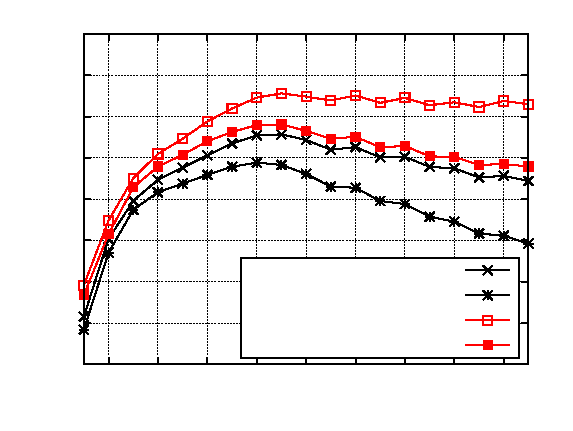
\includegraphics{./10.achievable_rates/img/Fig11}}%
    \gplfronttext
  \end{picture}%
\endgroup
